\documentclass[twoside]{article}

\usepackage{cite}
\usepackage{listings}

\usepackage[sc]{mathpazo} % Use the Palatino font
\usepackage[OT1]{fontenc} % Use 8-bit encoding that has 256 glyphs
\usepackage[utf8]{inputenc}
\linespread{1.05} % Line spacing - Palatino needs more space between lines
\usepackage{microtype} % Slightly tweak font spacing for aesthetics
\usepackage{graphicx}
\usepackage[round]{natbib}

\usepackage[hmarginratio=1:1,top=32mm,columnsep=20pt,left=2cm,right=2cm]{geometry} % Document margins
\usepackage{multicol} % Used for the two-column layout of the document
\usepackage[hang, small,labelfont=bf,up,textfont=it,up]{caption} % Custom captions under/above floats in tables or figures
\usepackage{booktabs} % Horizontal rules in tables
\usepackage{float} % Required for tables and figures in the multi-column environment - they need to be placed in specific locations with the [H] (e.g. \begin{table}[H])
\usepackage{hyperref} % For hyperlinks in the PDF

\usepackage{paralist} % Used for the compactitem environment which makes bullet points with less space between them

\usepackage{abstract} % Allows abstract customization
\renewcommand{\abstractnamefont}{\normalfont\bfseries} % Set the "Abstract" text to bold
\renewcommand{\abstracttextfont}{\normalfont\small\itshape} % Set the abstract itself to small italic text

\usepackage{titlesec} % Allows customization of titles
\renewcommand\thesection{\Roman{section}} % Roman numerals for the sections
\renewcommand\thesubsection{\Alph{subsection}}
\titleformat{\section}[block]{\large\scshape\centering}{\thesection.}{1em}{} % Change the look of the section titles
\titleformat{\subsection}[block]{\large}{\thesubsection.}{1em}{} % Change the look of the section titles

\graphicspath{{./images/}}

\usepackage{amsmath}

\title{\vspace{-15mm}\fontsize{24pt}{10pt}\textbf{Self-supervised learning from snaps}}

\author{
  \large
  \textsc{Kenneth Blomqvist}\\[2mm]
  \texttt{kenneth.blomqvist@aalto.fi}\\[2mm]
  \and
  \textsc{Aleksi Hämäläinen}\\[2mm]
  \texttt{aleksi.hamalainen@aalto.fi}\\[2mm]
}
\date{}

\newcommand{\norm}[1]{\left\lVert#1\right\rVert}

%----------------------------------------------------------------------------------------

\begin{document}

\maketitle % Insert title

%----------------------------------------------------------------------------------------
%	ABSTRACT
%----------------------------------------------------------------------------------------

\begin{abstract}
  This paper attempts to replicate results obtained in the paper `Time-Contrastive networks: self-supervised learning from video`. \citep{self-supervised-learning} We perform experiments to show that videos taken from a single viewpoint can be used to learn a distance preserving embedding of a scene onto a vector space. We attempt to teach a simulated robotic arm to imitate itself performing different trajectories using reinforcement learning and the learned embedding. The results show that an embedding can be learned in a self-supervised manner. However, learning to imitate proved itself more challenging.

%%% Local Variables:
%%% mode: latex
%%% TeX-master: "report"
%%% End:

\end{abstract}

%----------------------------------------------------------------------------------------
%	ARTICLE CONTENTS
%----------------------------------------------------------------------------------------

\begin{multicols}{2} % Two-column layout throughout the main article text

  \section{Introduction}
  \label{sec:introduction}
  
Learning from others is one of the primary ways in which animals, humans included, learn to perform new tasks. Augmenting robots with such learning capabilities could open up countless new applications for robots. It would be even more benefitial, if such learning could occur from simple videos of humans demonstrating a task. Collecting videos of humans performing a task is very simple and cheap to do.

In this project we attempt to replicate results from the paper titled `Time-contrastive networks: self-supervised learning from video` \cite{self-supervised-learning}. In the paper the authors propose a way to teach a robot manipulation tasks using videos of a human performing a task without an explicit supervision signal. Differences in the frames across time are used as a learning signal.

A distance preserving embedding is learned using a triplet loss function. This learned function is used to create a reward function for reinforcement learning of the task. The triplets used for training can be constructed using either video from multiple views or by using single-view video.

We attempt to replicate a simplified version of the problem. Namely, we try to teach a simulated robot to imitate itself performing different moves in a video taken from a single viewpoint.

Section \ref{sec:methods} presents the main ideas behind the methods used in the experiments. Section \ref{sec:experiments} presents the experiments we performed. Section \ref{sec:results} presents the results we obtained. Section \ref{sec:discussion} provides some subjective conclusions we draw from our experience building this project and our results.


%%% Local Variables:
%%% mode: latex
%%% TeX-master: "report"
%%% End:



  \section{Methods}
  \label{sec:methods}
  
Here we present the main methods utilized by our project.

\subsection{Learning an embedding}

The paper \cite{self-supervised-learning} presents a way to learn a distance preserving embedding from video frames onto an n-sphere. The goal is to map frames that are close to each other in the video to vectors that are close to each other on the n-sphere as measured by the $L_2$-norm.

The embedding function is denoted $f(x)$ where $x$ is a frame from a video. We use three types of frames: an anchor frame $x_a$, a positive frame $x_p$ and a negative frame $x_n$. The anchor frame is closer to the positive frame than the negative frame.

Essentially, we want the constraint \[
    \norm{f(x_a) - f(x_p)}^2_2 + \delta < \norm{f(x_a) - f(x_n)}^2_2
    \] to hold. $\delta$ is a constant margin parameter.

$f$ is a convolutional neural network. The network is optimized by optimizing a triplet loss function. \[
    L(x_a, x_p, x_n) = \delta + \norm{f(x_a) - f(x_p)}^2_2 - \\
    \norm{f(x_a) - f(x_n)}^2_2
    \]

The triplets are either from a single or multiple viewpoints. When using multiple viewpoints, the anchor frame is a random frame sampled from the video. The positive frame is a frame from the exact same time-step but another viewpoint than the anchor frame. The negative frame is a frame sampled from the same viewpoint as the anchor frame outside a margin range around the anchor frame. This enables the network to learn a viewpoint invariant representation of the scene. \citep{self-supervised-learning}

In the single viewpoint case, all frames are from the same viewpoint. The anchor frame is again a random frame of the video. The positive frame is within a small margin range of the anchor frame. The negative frame is from outside a larger margin range of the anchor frame. \citep{self-supervised-learning}

\subsection{Learning using reinforcement learning}

We learn to imitate using reinfocement learning. The reward function is defined using the embedding shown in the previous section.

We use a huber-style loss: \[
    R(\boldsymbol{v_t}, \boldsymbol{w_t}) = -\alpha \norm{\boldsymbol{w_t} - \boldsymbol{v_t}}^2_2 -\beta \sqrt{\gamma + \norm{\boldsymbol{w_t} - \boldsymbol{v_t}}^2_2}
\]

Here $\alpha$ and $\beta$ are scaling parameters. $\gamma$ is a small constant to make the equation well defined for almost zero distances. $\boldsymbol{w_t}$ is an embedding of an image of the robot itself and $\boldsymbol{v_t}$ is an embedding the example video frame at timestep t.

We learn a policy that optimizes the reward function using the proximal policy optimization algorithm (PPO) \citep{ppo}. PPO is a robust, simple, model free policy gradient algorithm. It optimizes a clipped loss function: \[
    L(\theta) = \hat{E}_t[\min{r_t(\theta)\hat{A}_t, clip(r_t(\theta), 1 - \epsilon, 1 + \epsilon)\hat{A}_t})]
\]
$r_t(\theta)$ is the ratio between the probability of the action taken under the current policy and the policy before the previous update. $\hat{A}_t$ is the advantage defined: \[
    \hat{A}_t = -V(s_t) + r_t + \gamma r_{t+1} + ... + \gamma^{T-t+1}r_{T-1} + \gamma^T V(s_T)
    \]

The policy and value functions are neural networks. This surrogate reward function can be updated using multiple epochs of minibatch updates, making it well suited for neural networks. \citep{ppo}




  \section{Experiments}
  \label{sec:experiments}
  
We are interested in two questions:
\begin{itemize}
\item Is it possible to learn an embedding of video frames in a self-supervised manner using only videos from a single viewpoint?
\item Is the learned embedding robust and well-behaved enough to power a reward function to use as part of a reinforcement learning problem?
\end{itemize}

\subsection{Embedding frames of a robotic arm}

We created 200 videos of a robotic arm performing trajectories in a simulated environment. The arm is initialized to random joint positions and it moves to goal joint positions which are also randomly sampled. We use the Bullet 3 physics simulator and a robot modelled after the Kuka iiwa robotic arm.

{
    \label{example-snap}
    \centering
    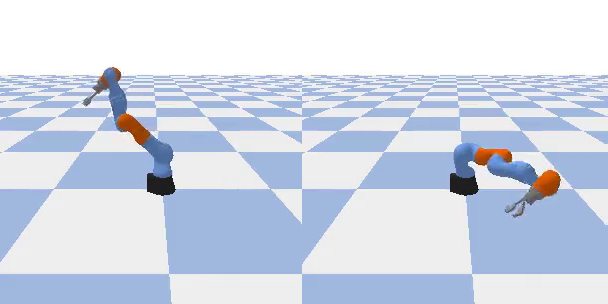
\includegraphics[width=8cm]{example_snap.png}
    \captionof{figure}{Two example frames from a recorded trajectory. The left frame is the goal position and the right frame is the start position.}
    \vspace{0.5cm}
}

We split the 200 videos such that 190 are used for training and 10 for validation.

We use a convolutional neural network derived from the Inception architecture as presented in \citep{inception-v3}. We use the 8 first layers of the network up until the layer labeled `Mixed\_5d`. We add two batch normalized convolutional layers, one spatial softmax transformation followed by two fully connected layers. This is very similar as the network used in \cite{self-supervised-learning}.

The network was implemented using the PyTorch deep learning framework. The layers taken from the inception architecture are initialized to values pretrained on the ImageNet dataset. The added layers are randomly initialized using the default initialization scheme of the PyTorch package.

In our experiments, the output of the network is a 32-dimentional embedding constrained to have an $L_2$ norm of 10. The scaling factor of 10 was motivated by results presented in \cite{constrained-softmax-loss}. We use a margin value of 2.0. The positive frame was sampled from within 10 frames of the anchor frame. The negative frame was sampled from outside a range starting from 30 frames before the anchor frame and ending 30 frames after the anchor frame. The size of the video is 299

We use the triplet loss presented in the previous section. At each epoch, we create a dataset of triplets sampled from 5 videos with 200 samples per video. We then run stochastic gradient descent with momentum against the triplet loss over this dataset 5 times after which a new triplet dataset is sampled and the process is repeated. The use a batch size of 64 triplets.

We use a learning rate schedule such that we start with a learning rate of 0.1. Each 500 epochs we decrease the learning rate to 1/10th of the previous rate until we reach 0.0001 inclusive.

% Please add the following required packages to your document preamble:
{
    \vspace{0.5cm}
    \centering
    \label{cnn-params}
    \begin{tabular}{@{}ll@{}}
    \toprule
    \textbf{Parameter}             & \textbf{Value}    \\ \midrule
    \textbf{minibatch size}        & 64                \\
    \textbf{learning rate}         & 0.1-0.0001        \\
    $\boldsymbol{\delta}$                & 2.0               \\
    \textbf{positive frame margin} & 10                \\
    \textbf{negative frame margin} & 30                \\
    \textbf{optimizer}             & SGD with momentum \\
    \textbf{momentum}              & 0.9               \\
    \textbf{embedding dimensions}  & 32
    \end{tabular}
    \captionof{table}{The parameters we used for training our embedding function.}
}

\subsection{Learning to imitate}

We used the learned embedding to teach the same simulated robot to imitate itself in a video performing different trajectories. We use the proximal policy optimization algorithm to optimize the loss function.

The observation at each time step is a concatenation of the robot joint states, joint velocities, the TCN embedding of an image of itself and the TCN embedding of the video frame at that timestep.

The reward is calculated using the huber loss presented in section \ref{sec:methods} using the embedding of an image of the robot and the embedding of an example video frame. Actions are torques applied to the 12 joints of the robotic arm.




  \section{Results}
  \label{sec:results}
  
We monitored the accuracy of our embeddings over the course of training our CNN. The validation set is a dataset of 1000 triplets such that 100 triplets are created from each of the 10 validation videos. After the end of training, 736/1000 samples fulfilled the triplet constraint. 930/1000 fulfilled the contrained without the added margin. I.e. $\norm{x_a - x_p} < \norm{x_a - x_n}$.

For comparison after 10 epochs of training the values were 467/1000 with margin and 894/1000 without the margin.

{
    \centering
    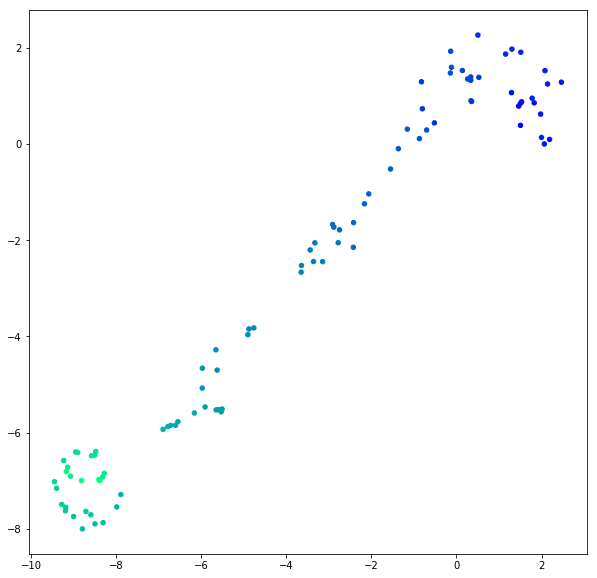
\includegraphics[width=8cm]{t-sne-trajectory.png}
    \captionof{figure}{A t-SNE plot of a validation trajectory. Perplexity 30, learning rate 200 and 1000 iterations. The color goes from blue to cyan as a function of the frame indices.}
    \label{t-sne}
    \vspace{0.25cm}
}

The t-SNE plot in figure \ref{t-sne} of a validation trajectory suggests that the network has learned a meaningful and well-behaved embedding of the video frames. Embeddings of frames that are close to each other in the video are close to each other in the dimensionality reduced regime.

{
    \centering
    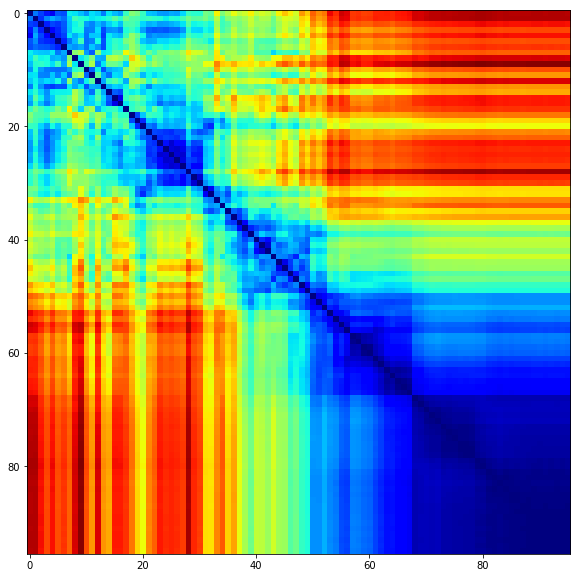
\includegraphics[width=8cm]{dima.png}
    \captionof{figure}{Visualization of the $L_2$ distance matrix of the same validation video as in figure \ref{t-sne}. Blue means close and red is far away.}
    \label{dima}
    \vspace{0.25cm}
}

{
    \centering
    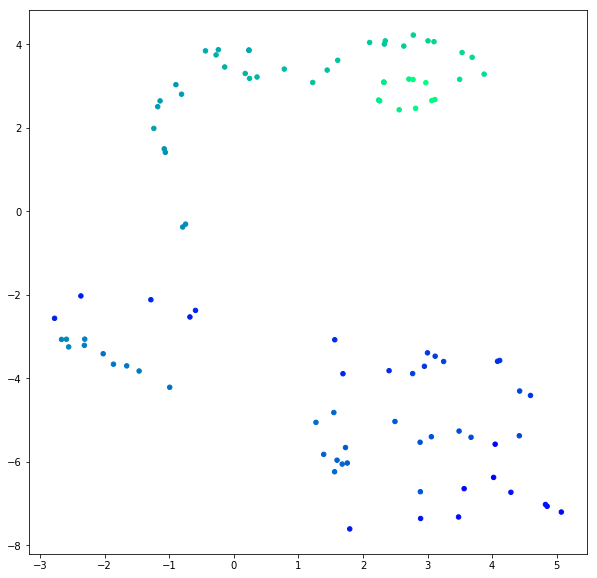
\includegraphics[width=8cm]{early_trajectory.png}
    \captionof{figure}{For comparison, a visualization of a trajectory after 50 epochs of training. Visualized using the same t-SNE parameters and the same video as figure \ref{t-sne}.}
    \label{early-t-sne}
    \vspace{0.25cm}
}
{
    \centering
    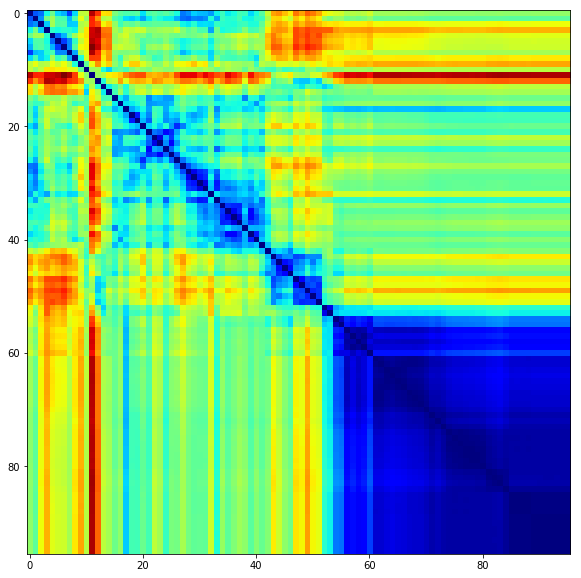
\includegraphics[width=8cm]{early-dima.png}
    \captionof{figure}{Distance matrix for the same network as in figure \ref{early-t-sne}.}
    \label{early-dima}
    \vspace{0.25cm}
}

Each row and column in the distance matrix shown in figure \ref{dima} corresponds to a frame of the video. The value is the euclidean distance between the embedding of the frame. I.e. the diagonal is 0 and the matrix is symmetric. This visualization seems to confirm that subsequent frames are close to each other in the embedding space.

Comparing figure \ref{t-sne} to figure \ref{early-t-sne} and figure \ref{dima} to figure \ref{early-dima} we can see that early on in training the network has not yet learned a meaningful embedding of the entire joint space of the robot.

First, we studied performance of the PPO algorithm to generate trajectories in a simplified environment where a task is to move the robotic arm into a randomly sampled goal position. Reward of the problem is $L_2$ norm of the distance between a goal position and a robot arm position at a time step. The experiment indicates that the complexity of the problem is high. Figure \ref{trajectory_learning} shows learning results of the experiment. The PPO algorithm learns to generate better trajectories. However, as the reward at the end of iterations show the agent accomplish to build correct trajectories for only portion of the sampled goal positions.

{
    \centering
    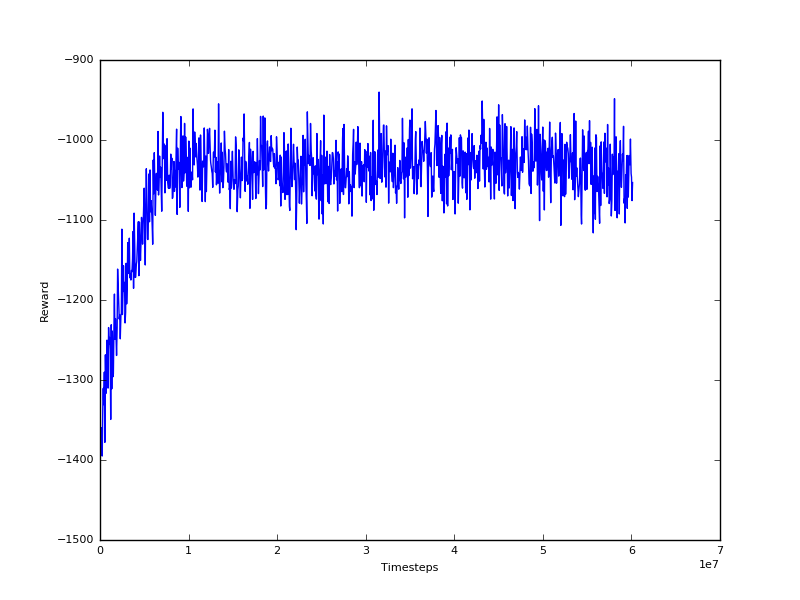
\includegraphics[width=10cm]{modified_model_1.png}
    \captionof{figure}{Learning of the trajectory pose problem}
    \label{trajectory_learning}
    \vspace{0.25cm}
}

As moving the robot arm to a randomly sampled position proved to be challenging, no remarkable achievements were expected for the imitation learning task. Hence, we experimented the imitation problem with one example video. Figure \ref{imitation} shows the achieved learning. The PPO algorithm produces trajectories that have similar features as the example video. For example, the ending pose is close to the example pose especially if we take into account that viewing angles differ. However, in the middle of the movement the position clearly differs from the example.

{
    \centering
    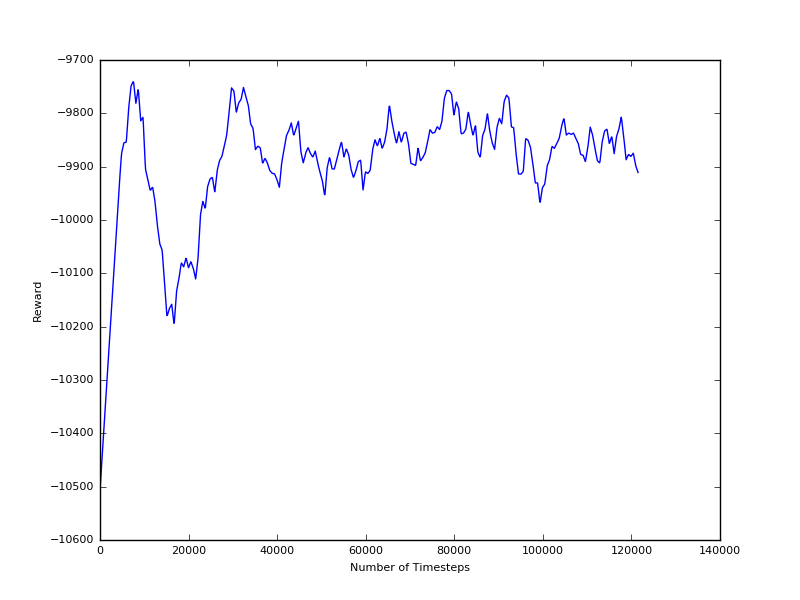
\includegraphics[width=10cm]{imitation_1.png}
    \captionof{figure}{Learning of the Imitation problem}
    \label{imitation}
    \vspace{0.25cm}
}

  \section{Discussion}
  \label{sec:discussion}
  
As we have seen, it is possible to learn a meaningful embedding of video frames taken from a single viewpoint onto a vector space. Computer vision has progressed a lot in recent years and methods such as convolutional neural networks have become very usable with tools such as PyTorch. Implementing the neural network and tuning the parameters did not prove to be very difficult.

Learning to imitate was more of a challenge. We performed many runs of our experiments, but ultimately failed to learn any useful behaviour. This might be due to areas in the domain of our embedding function which are not properly mapped onto the codomain. It might be that these areas were not properly represented in our training data.

Proximal policy optimization is known to not be very sample efficient. One hypothesis might be that we simply did not train our policy and value functions for long enough or that we did not manage to find suitable parameters for the algorithm. We can not entirely rule out that there are no bugs in our code. However, we did try our implementation on more simple environments from the Openai gym \citep{gym}. We also tried the PPO algorithm in our simulation on a different environment where the objective is to move the robotic arm into a randomly sampled goal position. The state in this environent was the goal position, the robot joint states and velocities. In these simpler environments the algorithm appeared to learn adequately.

A model-based reinforcement learning algorithm could probably learn faster to master the task of learning to perform trajectories.

It would be interesting to run our imitation experiments using more computational resources than we had available. Another interesting experiment would be to try and use videos taken from multiple viewpoints.





  %	REFERENCE LIST
  %----------------------------------------------------------------------------------------

  \bibliographystyle{plainnat}
  \bibliography{references}

\end{multicols} % One-column layout for the appendices
\pagebreak

%----------------------------------------------------------------------------------------

\end{document}

%%% Local Variables:
%%% mode: latex
%%% TeX-master: t
%%% End:
